\documentclass[12pt]{revtex4-2}
\usepackage[utf8]{inputenc}

\usepackage{amsthm}
\usepackage{amsmath}
\usepackage{amsfonts}
\usepackage{amssymb}
\usepackage{graphicx}
% \usepackage{natbib}
\usepackage{listings}
\usepackage{verbatim}
\usepackage[margin=1in]{geometry}
\setlength{\parindent}{0pt}

\newcommand{\R}{\mathbb{R}}
\newcommand{\C}{\mathbb{C}}
\newcommand{\N}{\mathbb{N}}
\newcommand{\Z}{\mathbb{Z}}
\newcommand{\Q}{\mathbb{Q}}
\newcommand{\real}{\text{Re}}
\newcommand{\imag}{\text{Im}}
\newcommand{\Tr}{\text{Tr}}

\begin{document}

\title{Notes on: Quantum Oscillations}
\author{Joseph Roll}
\affiliation{University of Texas at Austin}

\begin{abstract}
    These notes help gain some insight into quantum oscillations\textemdash the reasoning behind how researchers use magnetic fields to experimentally determine Fermi surfaces.  It is the explanation for the de Haas-van Alphen effect (oscillating magnetic susceptibility), and similar ones such as the Shubnikov-de Haas effect (oscillating resistivity).  We start with some preliminary classical electromagnetic theory, then we look specifically at its effects on electrons in metals through canonical quantization.
\end{abstract}

\maketitle

\section{Derivation of minimal coupling}
\subsection{Classical regime}

It is common knowledge (after taking a course in quantum mechanics) that to consider a quantum system with an external magnetic field we use minimal coupling; all momentum operators are mapped $\hat{\mathbf{p}} \mapsto \hat{\mathbf{p}} - q\hat{\mathbf{A}}$ where $\nabla \times \mathbf{A} = \mathbf{B}$.  However, it is important to remind ourselves why we can do this in the first place.  Its origins are actually not within quantum mechanics, but from classical mechanics (Lagrangian and Hamiltonian formalisms) and classical electromagnetism (Maxwell's equations and the Lorentz force).
\par
From Gauss' law, we know how there are no magnetic monopoles:  $\nabla \cdot \mathbf{B} = 0$.  This implies the existence of some vector potential $\mathbf{A}$ such that $\mathbf{B} = \nabla \times \mathbf{A}$.  We can use this with Faraday's law to look at our electric field.
\begin{align}
    0 &= \nabla \times \mathbf{E} + \frac{\partial \mathbf{B}}{\partial t} \\
    &= \nabla \times \mathbf{E} + \frac{\partial}{\partial t}(\nabla \times \mathbf{A}) \\
    &= \nabla \times \left(\mathbf{E} + \frac{\partial\mathbf{A}}{\partial t} \right).
\end{align}

Therefore there exists a scalar potential $\varphi$ such that $\mathbf{E} + \partial_t\mathbf{A} = -\nabla\varphi$.  So $\mathbf{E} = -\nabla\varphi - \partial_t\mathbf{A}$.  Applying this to the Lorentz for some charged particle (with charge $q$ and mass $m$), Newton's second law states
\begin{align}
    \mathbf{F} = m\ddot{\mathbf{x}} &= q\mathbf{E} + q\mathbf{v}\times\mathbf{B} \\
    &= -q\nabla\varphi - q\frac{\partial \mathbf{A}}{\partial t} + q\mathbf{v}\times(\nabla \times \mathbf{A}).
\end{align}

We can also rewrite the central term on the RHS with the chain rule.
\begin{equation}
    \frac{d\mathbf{A}}{dt} = \frac{\partial \mathbf{A}}{\partial t} + \sum_i \frac{\partial x_j}{\partial t}\frac{\partial \mathbf{A}}{\partial x_j} = \frac{\partial \mathbf{A}}{\partial t} + (\mathbf{v} \times \nabla)\mathbf{A} \implies \frac{\partial \mathbf{A}}{\partial t} = \frac{d\mathbf{A}}{dt} - (\mathbf{v} \cdot \nabla)\mathbf{A}.
\end{equation}

This actually helps us if we rewrite the rightmost term on the RHS.  We could either use a vector identity, or use the Levi-Civita tensor to quickly see where it comes from.
\begin{align}
    \big[\mathbf{v}\times(\nabla \times \mathbf{A})\big]_i &= \varepsilon_{ijk}v_j(\nabla \times \mathbf{A})_k \\
    &= \varepsilon_{ijk}v_j\varepsilon_{kmn}\partial_m A_n \\
    &= \varepsilon_{ijk}\varepsilon_{mnk}v_j\partial_m A_n \\
    &= (\delta_{im}\delta_{jn} - \delta_{in}\delta_{jm})v_j\partial_m A_n \\
    &= v_j\partial_i A_j - v_j\partial_j A_i \\
    &= \partial_iv_j A_j - v_j\partial_j A_i \\
    &= \big[ \nabla(\mathbf{v} \cdot \mathbf{A}) \big]_i - \big[ (\mathbf{v}\cdot\nabla) \mathbf{A} \big]_i \\
    \mathbf{v}\times(\nabla \times \mathbf{A}) &= \nabla (\mathbf{v} \cdot \mathbf{A}) - (\mathbf{v}\cdot\nabla) \mathbf{A}.
\end{align}

Substituting these back into our equation of motion yields
\begin{align}
    m\ddot{\mathbf{x}} &= -q\nabla\varphi - q\left[ \frac{d\mathbf{A}}{dt} - (\mathbf{v} \cdot \nabla)\mathbf{A} \right] + q\left[ \nabla(\mathbf{v} \cdot \mathbf{A}) - (\mathbf{v}\cdot\nabla) \mathbf{A} \right] \\
    &= q\left[ -\nabla\varphi - \frac{d\mathbf{A}}{dt} + \nabla(\mathbf{v} \cdot \mathbf{A}) \right] \\
    &= q\left[ -\nabla\left( \varphi - \mathbf{v}\cdot\mathbf{A} \right) - \frac{d\mathbf{A}}{dt} \right]. \label{eqn:em-eom}
\end{align}

The goal now is to use this to use this to find some potential $U$ which generates this force, however we are not guaranteed to satisfy $\mathbf{F} = -\nabla U$ here because the velocity component of our force means it is not a conservative vector field!  Instead, we need some $U$ such that [Goldstein Page 21]
\begin{equation}
    F_j = -\frac{\partial U}{\partial x_j} + \frac{d}{dt}\left( \frac{\partial U}{\partial \dot{x}_j} \right). \label{eqn:nonconservative-pot}
\end{equation}

Looking at our prior expression for the force, we are actually super close to this form.  We need to note how $\varphi = \varphi(\mathbf{x})$ and $\mathbf{A} = \mathbf{A}(\mathbf{x})$ are not velocity dependent.  Then
\begin{equation}
    A_i = \frac{\partial}{\partial \dot{x}_i}\left( \sum_j\dot{x}_j A_j - \varphi \right) \implies \frac{dA_i}{dt} = \frac{d}{dt}\left[ \frac{\partial}{\partial \dot{x}_i}\big( \mathbf{v}\cdot \mathbf{A} - \varphi \big) \right].
\end{equation}

which uses the fact that $\partial x_i/\partial x_j = \delta_{ij}$. Substituting this into Eqn \ref{eqn:em-eom} yields
\begin{equation}
    m\ddot{x_i} = q\left\{ -\frac{\partial}{\partial x_i}\big( \varphi - \mathbf{v}\cdot\mathbf{A} \big) + \frac{d}{dt}\left[ \frac{\partial}{\partial \dot{x}_i}\left( \varphi - \mathbf{v}\cdot\mathbf{A} \right) \right] \right\}.
\end{equation}

This is the exact form of our generatized potential function (Eqn. \ref{eqn:nonconservative-pot})!
\begin{equation}
    U = q\varphi - q\mathbf{v}\cdot\mathbf{A}.
\end{equation}

Our Lagrangian is then 
\begin{equation}
    \mathcal{L} = T - U = \frac{1}{2}m \mathbf{v}\cdot\mathbf{v} - q\varphi + q\mathbf{v}\cdot\mathbf{A}.
\end{equation}

Recall that the canonical momentum (review Legendre transforms if this is unfamiliar) is
\begin{equation}
    p_i = \frac{\partial \mathcal{L}}{\partial \dot{x}_i} = m\dot{x}_i - qA_i.
\end{equation}

Thus, when we want to apply some magnetic field to a charged particle in the Hamiltonian formalism, we do so by the mapping
\begin{equation}
    \boxed{\mathbf{p} \mapsto \mathbf{p} - q\mathbf{A}}
\end{equation}

\subsection{Quantum regime}

This has all been in the classical regime, though, and the name of the notes is \em quantum \em oscillations.  To go from classical to quantum particles, there are two main approaches:
\begin{enumerate}
    \item Canonical quantization
    \item Path integrals
\end{enumerate}

The path integral formulation is more mathematically sound/rigorous, but is much more complicated.  For the sake of convenience, and the fact that I do not know path integrals very well, we will use canonical quantization.  There are several axioms within the canonical quantization framework, which are outlined well in \textit{Geometry, Topology, and Physics} by Nakahara in Section 1.2.2.  

However, here we will just have our classical position and momentum variables map to operators $x \mapsto \hat{x}$ and $p \mapsto \hat{p}$, have that 
\begin{equation}
    [\hat{x}_j,\hat{x}_k] = 0 \qquad [\hat{p}_j,\hat{p}_k]  \qquad [\hat{x}_j,\hat{p}_k] = i\hbar \delta_{jk}
\end{equation}

and have these operators work like one would imagine for a quantum system.  Thus for our purposes, working with electrons, it is common to work with
\begin{equation}
    \boxed{ \hat{\vec{\pi}} := \hat{\mathbf{p}} + e\mathbf{A} }
\end{equation}

% For the sake of completeness, it is also important to note that while we have $[\hat{x}_i,\hat{\pi}_j] = i\hbar \delta_{ij}$ (since $[\hat{x}_i,A_j(\hat{\mathbf{x}})] = 0$), we also have
% \begin{align}
%     [\hat{\pi}_j,\hat{\pi}_j] &= [\hat{p}_j + eA_j , \hat{p}_k + eA_k] \\
%     &= e[\hat{p}_j,A_k] + e[A_j,\hat{p}_k] \\
%     &= e\hat{p}_jA_k - eA_k\hat{p}_j + eA_j\hat{p}_k - e\hat{p}_kA_j \\
%     &= e(\partial_jA_k) - e(\partial_k A_j).
% \end{align}

% This last equality uses the fact that, in the position basis, we have $\hat{p}_j = \partial/\partial x_j := \partial_j$.  It also takes care of our rightmost differential operators by using a test function $f$ on both sides.  Through the product rule $\partial_j(A_k f) = (\partial_j A_k)f + A_k(\partial_j f)$, our two central terms vanish.  Then we have
% \begin{equation}
%     \partial_j A_k - \partial_k A_j = \epsilon_{jki}(\nabla \times \mathbf{A})_i.
% \end{equation}

% Therefore, with slightly more familiar indexing, we have $[\hat{\pi}_i,\hat{\pi}_j] = \epsilon_{ijk}B_k \neq 0$.  While this is not too critical for these notes, it is still important to realize that we cannot treat $\hat{\vec{\pi}}$ \em exactly \em like our typical momentum because of this.

\newpage
\section{Landau levels and landau tubes}

\subsection{Deriving our hamiltonian}

Note that henceforth we will denote the applied external magnetic field as $\mathbf{H}$, its magnitude as $|\mathbf{H}| = H$, and the Hamiltonian as $\hat{H}$.
\par

As outlined in the prior section, we will be working with (quantum) electrons in an external magnetic field $\mathbf{H} = (0,0,H)$; this uses the standard cartesian coordinates for real space.  To use minimal coupling, we need to choose some vector potential to achieve this magnetic field.  Thanks to the gauge invariance of $\nabla \times (\nabla f) = 0 \implies \nabla \times \mathbf{A} = \nabla \times (\mathbf{A} + \nabla f) $, for some scalar field $f$, we have some freedom in this choice.  Let $\mathbf{A} = (0,Hx,0)$.  We can quickly verify how
\begin{equation}
    \nabla \times \mathbf{A} = \begin{vmatrix}
        e_1 & e_2 & e_3 \\
        \partial_x & \partial_y & \partial_z \\
        0 & Hx & 0
    \end{vmatrix} = (0,0,H).
\end{equation}

As our vector potential only has a $y$ component, our Hamiltonian is given by
\begin{equation}
    \hat{H} = \frac{p_x^2}{2m_e} + \frac{(p_y + eHx)^2}{2m_e} + \frac{p_z^2}{2m_e}.
\end{equation}

Since $\hat{H}$ is not a function of $y$, we have $[\hat{H},p_y] = 0$; so we can replace all $p_y$ operators with its eigenvalue of $\hbar k_y$.  Quickly justifying this fact, note that since $[\hat{H},p_y] = 0$ there exists some basis that diagonalizes both $\hat{H}$ and $y$.  Then we know our eigenvalue is $\hbar k_y$ since $p_y = -i\hbar\partial_y$ leads to an exponential wavefunction $A(x,z)e^{i yk_y}$.
\begin{align}
    \hat{H} &= \frac{p_x^2}{2m_e} + \frac{(\hbar k_y + eHx)^2}{2m_e} + \frac{p_z^2}{2m_e} \\
    &= \frac{p_x^2}{2m_e} + \frac{1}{2}m\left( \frac{eH}{m_e} \right)^2 \left[x + \frac{\hbar k_y}{m_e} \left( \frac{m_e}{eH} \right) \right]^2 + \frac{p_z^2}{2m_e} \\
    &= \left[ \frac{p_x^2}{2m_e} + \frac{1}{2}m_e\omega_c^2\left( x + \frac{\hbar k_y}{m_e\omega_c} \right)^2 \right] + \frac{p_z^2}{2m_e} \qquad : \qquad \omega_c := \frac{eH}{m_e}.
\end{align}

This term in square brackets is just the quantum harmonic oscillator (QHO) with frequency $\omega_c$ and a position offset of $-\hbar k_y/m_e\omega_c$.  Thus we can rewrite it as
\begin{equation}
    \boxed{ \hat{H} = \hbar\omega_c\left( n + \frac{1}{2} \right) + \frac{p_z^2}{2m_e} }
\end{equation}

for some $n \in \N_0$.

\subsection{Degeneracy of landau levels}
Note that the possible values of our eigenvalue $p_y \mapsto \hbar k_y$ depend on the physical system.  This comes from us actually working with a discrete system, so this plane wave is from the discrete Fourier transform of our real-space sample: $k_y = 2\pi N/L_y$ for $N \in \N$.  Then since our QHO is shifted in real space by $\hbar k_y/m_e\omega_c$, it must still lie within our sample.
\begin{gather}
    0 \leq \frac{\hbar k_y}{m_e\omega_c} \leq L_x \\
    0 \leq \frac{2\pi N}{L_y} < \frac{m_e\omega_c}{\hbar}L_x \\
    0 \leq N < \frac{m_e\omega_c}{2\pi\hbar} L_xL_y.
\end{gather}

If $\Phi_0 := h/e$ is our fundamental flux quanta and $\Phi := HA = HL_xL_y$ is the net magnetic flux of our system, then our upper limit here becomes
\begin{equation}
    \frac{m_e\omega_c}{2\pi\hbar}L_xL_y = \frac{m_eeB}{hm_e}L_xL_y = \frac{HL_xL_y}{h/e} = \frac{\Phi}{\Phi_0}.
\end{equation}

Then since electrons are spin-1/2 particles, each point in $k$-space has two states.  Thus we have $\boxed{ D = 2\Phi/\Phi_0 }$ states per flux quanta through our system.

\subsection{Area quantization and tube formation}
In the end, we can think of this mapping onto the QHO as setting
\begin{equation}\label{eqn:area_start}
    \frac{\hbar^2}{2m_e}(k_x^2 + k_y^2) = \hbar\omega_c\left( n + \frac{1}{2} \right).
\end{equation}

This is a circle in $(k_x,k_y)$ phase space with an area of
\begin{equation}
    A_n = \pi r_n^2 = \pi\hbar\omega_c\left( n + \frac{1}{2} \right)\frac{2m_e}{\hbar^2} \implies \boxed{ A_n = \frac{2\pi eH}{\hbar}\left( n + \frac{1}{2} \right)}\label{eqn:area-n}
\end{equation}

We can see how this are tubes though by fixing our energy $\epsilon$.  Our occupied states satisfy
\begin{align}
    \hbar\omega_c\left( n + \frac{1}{2} \right) + \frac{\hbar^2 k_z^2}{2m_e} &\leq \epsilon \\
    \frac{\hbar^2 k_z^2}{2m_e} &\leq \epsilon - \hbar\omega\left( n + \frac{1}{2} \right) \\
    k_z^2 &\leq \frac{2m_e}{\hbar^2}\left[ \epsilon - \hbar\omega\left( n + \frac{1}{2} \right) \right].
\end{align}

This bounds our $k_z$ values above and below; with our quantized area for $(k_x,k_y)$, we have our tube.

\newpage
\section{Electron orbits in metals}
\subsection{Cyclotron frequency and effective mass}
When we think of electrons in an external magnetic field, we will often define a cylcotron frequency $\omega_c = eH/m_e$ as we did in Section IIA.  This, however, is for a bare electron and is traveling in a circle (or helix).  In metals, we, by definition, have a Fermi surface (FS) which is not guaranteed to be circular.  Our electron will travel on a cut of our FS, as shown below, so we will need to define a new frequency.  It is of the same form as our prior cyclotron frequency with an effective mass; we find this effective mass in this subsection.
\par

Recall how our momentum is $\mathbf{p} = \hbar\mathbf{k}$.  So our Lorentz force (Newton's second law with $\mathbf{F} = \dot{\mathbf{p}}$) has
\begin{equation}\label{eqn:lorentz-force}
    \hbar\dot{\mathbf{k}} = -e (\mathbf{v} \times \mathbf{H}) \iff \hbar\frac{d\mathbf{k}}{dt} = -e\left( \frac{d\mathbf{r}}{dt} \times \mathbf{H} \right).
\end{equation}

Since the Lorentz force here is perpendicular to $\mathbf{v}$, it does no work on our electron.  Thus our energy is constant along our orbit as $\mathbf{k}$ changes with time.  We also need to recall that $\mathbf{v} = \hbar^{-1}\nabla_\mathbf{k}\epsilon_\mathbf{k}$ [Appendix A].  From this, we know that our velocity is normal to our constant energy cut.  Since $\dot{\mathbf{k}}$ is also perpendicular to $\mathbf{H}$, from our Lorentz force cross product, \underline{our electron must trace the intersection of our FS and the plane normal to $\mathbf{H}$}.  If we integrate Eqn. \ref{eqn:lorentz-force} with respect to time, 
\begin{equation}
    \hbar(\mathbf{k} - \mathbf{k}_0) = -e(\mathbf{r} - \mathbf{r}_0)\times\mathbf{H} \implies \hbar|\mathbf{k} - \mathbf{k}_0| = e|\mathbf{r} - \mathbf{r}_0||\mathbf{H}|\sin\theta.
\end{equation}

We want to see the components of our electron position projected onto the plane normal to $\mathbf{H}$, denoted $\mathbf{r}'$, which simply sets $\theta = 90^\circ$.
\begin{equation}
    \frac{\hbar}{eH}|\mathbf{k} - \mathbf{k}_0| = |\mathbf{r}' - \mathbf{r}'_0|.
\end{equation}

The time it takes our electron to trace $\mathbf{r}'$ will define our cyclotron frequency, and we can determine that below from our electronic structure. Taking the norm of Eqn. \ref{eqn:lorentz-force}, we get 
\begin{equation}
    dt = \frac{\hbar}{e} \frac{|d\mathbf{k}|}{|\mathbf{v}\times\mathbf{H}|} = \frac{\hbar^2}{e} \frac{|d\mathbf{k}|}{|\nabla_\mathbf{k}\epsilon \times \mathbf{H}|} = \frac{\hbar^2}{eH} \frac{dk}{|\nabla_\mathbf{k}\epsilon|}.
\end{equation}

The last equality is true as the electron orbit is in the normal plane to $\mathbf{H}$, we know $\nabla_\mathbf{k}\epsilon$ and $\mathbf{H}$ are perpendicular; also denote $|\mathbf{H}| = H$ and $|d\mathbf{k}| = dk$.  We can now take the component of our gradient that is normal to our FS and call it $\Delta k_n'$, see Fig. \ref{fig:fermi-surface}.  Then we can call the change in energy going slightly normal to our FS $\Delta \epsilon$.  So 
\begin{equation}
    dt = \frac{\hbar^2}{eH} \frac{dk}{(\Delta \epsilon / \Delta k_n')} = \frac{\hbar^2}{eH} \frac{\Delta k_n' dk}{\Delta \epsilon}.
\end{equation}

\begin{figure}[tb]
\centering
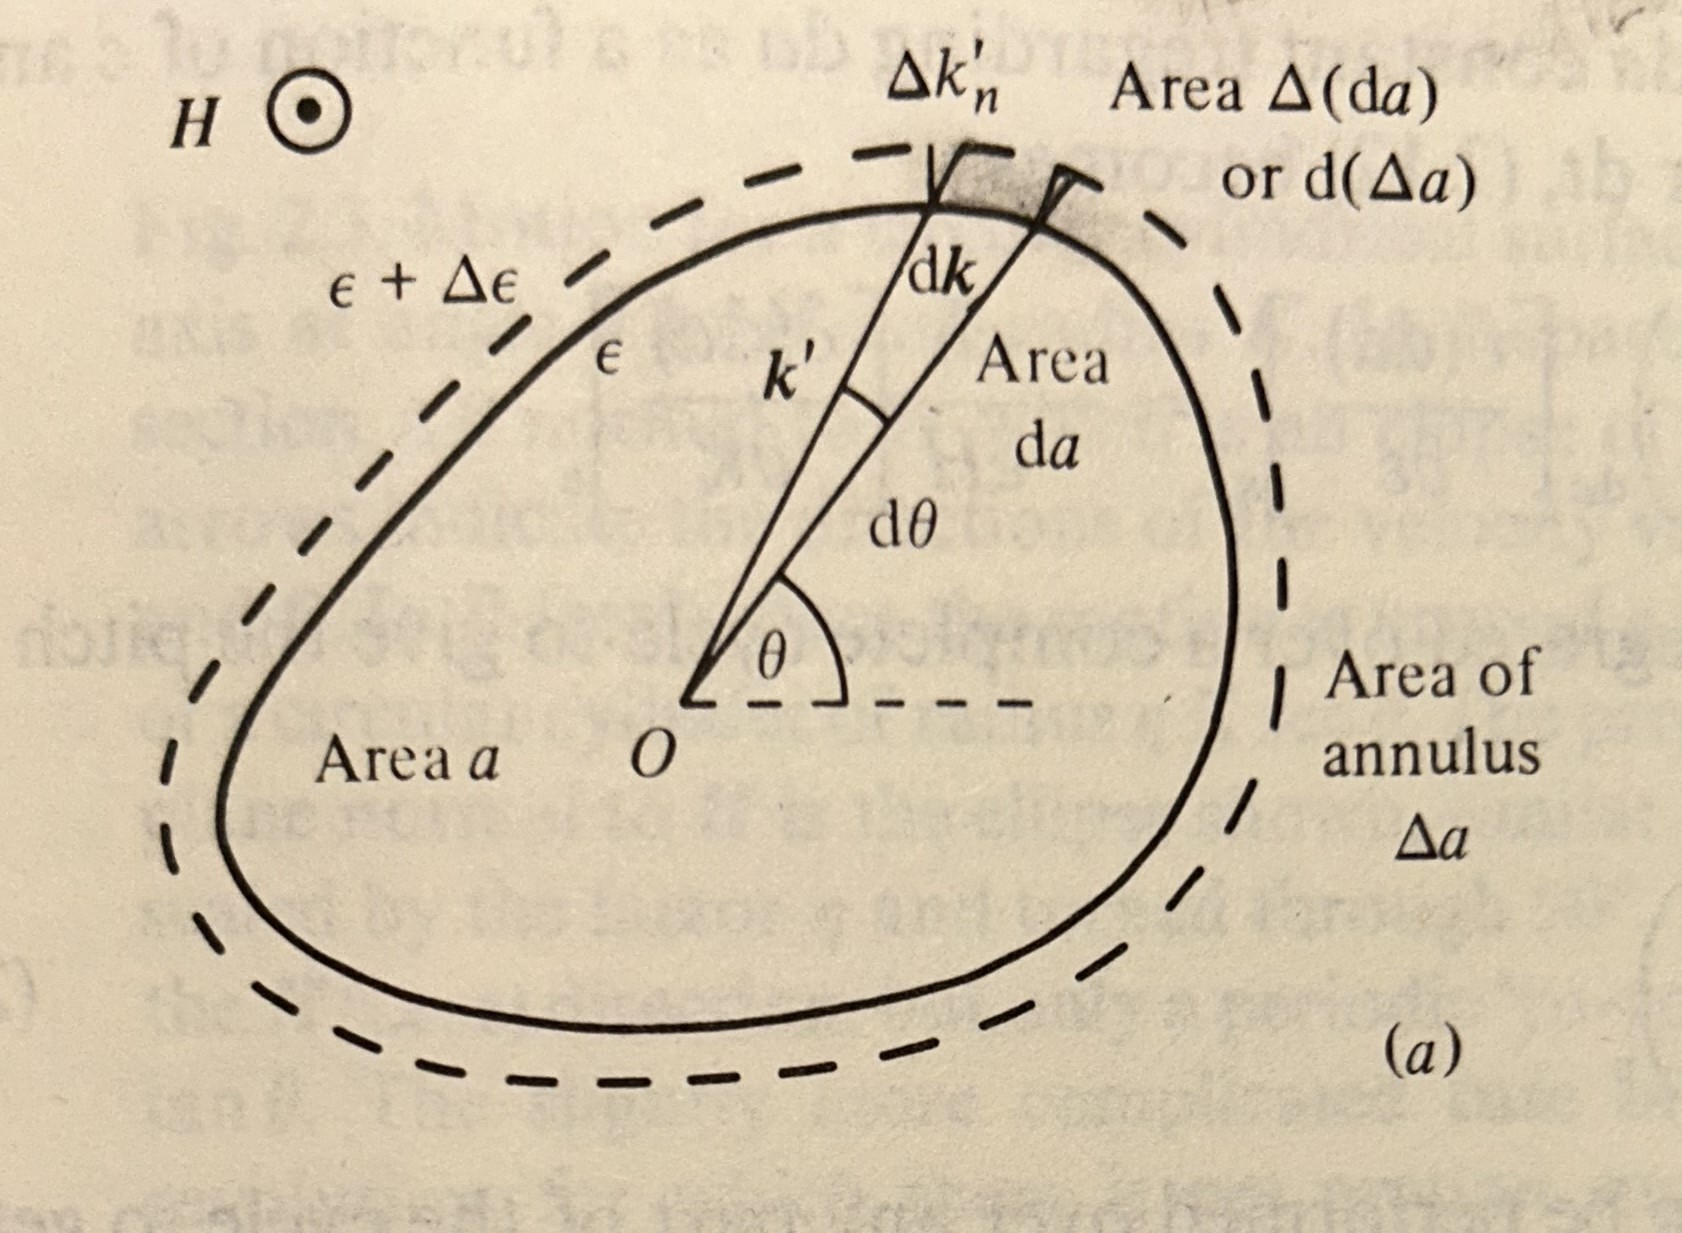
\includegraphics[width=0.5\textwidth]{figures/fermi_surface.jpg}
\caption{Generic fermi surface, which outlines how exactly we are defining our variables.  Taken from \textit{Magnetic Oscillations in Metals}.}
\label{fig:fermi-surface}
\end{figure}

Looking at our (rightmost) numerator, $\Delta k_n' dk$ represents an infinitesimal piece of area in $\mathbf{k}$-space from our annulus going from $\epsilon \to \epsilon + \Delta\epsilon$.  Thus we can set $\Delta k_n' dk \to d(\Delta a)$.  We also have $d(\Delta a) = \Delta(da)$ where $da$ integrating this infinitesimal will give our FS area.  Applying this to our prior expression yields
\begin{equation}
    dt = \frac{\hbar^2}{eH} \frac{\Delta (da)}{\Delta \epsilon} = \frac{\hbar^2}{eH}\left( \frac{\partial(da)}{\partial\epsilon} \right)_\kappa.
\end{equation}

We can then integrate over an entire electron oscillation.  The left will have $dt \to T$ be our period and the right will have $da \to A$ be our FS area.  Since our cyclotron frequency is an angular frequency, we have 
\begin{equation}
    T = \frac{2\pi}{\omega_c} = \frac{\hbar^2}{eH}\left( \frac{\partial A}{\partial\epsilon} \right)_\kappa \implies \omega_c = \frac{2\pi eH}{ \hbar^2}\left( \frac{\partial A}{\partial\epsilon} \right)_\kappa^{-1}.
\end{equation}

This also invites the definition for our effective mass, denoted $m$,
\begin{equation}
    \boxed{\omega_c = \frac{eH}{m} \qquad : \qquad m := \frac{\hbar^2}{2\pi}\left(\frac{\partial A}{\partial \epsilon}\right) }
\end{equation}

\subsection{Degeneracy of landau tubes}
Importantly, and done in the text I am following, we can rewrite our energy as 
\begin{equation}
    \epsilon = \left( n + \frac{1}{2} \right)\beta_e H + \frac{\hbar^2\kappa^2}{2m}
\end{equation}

where $\beta_e$ is the double Bohr magneton defined as $\beta := e\hbar/m_e$, and $\kappa := k_z$.  Redefining these more closely follows the texts I am referencing.  

Thus we can also Eqn. \ref{eqn:area_start} as
\begin{equation}
    \frac{\hbar^2}{2m_e}(k_x^2 + k_y^2) = \left(n + \frac{1}{2}\right)\beta_e H.
\end{equation}

Experimentally, we can see how the required quantum number $n$ here is extremelly large. This makes things a bit nicer as we can reasonably approximate differences of $n$ by differentiation (the same change if $n$ were tiny, but a smaller percentange change).  Thus we can see how successive energies yield
\begin{equation}
    (\Delta\epsilon)_{\Delta n=1} \approx \left( \frac{\partial\epsilon}{\partial A} \right)_\kappa (\Delta A)_{\Delta n=1} = \frac{1}{(\partial A/\partial \epsilon)_\kappa}\frac{2\pi eH}{\hbar} = \frac{2\pi e}{\hbar(\partial A/\partial \epsilon)_\kappa}H = \beta H
\end{equation}

where our subscript on derivatives here follows standard from statistical mechanics (subscript is what we assume constant).  Also note that our definition of $\beta$ here is just like our prior double Bohr magneton but with the effective mass instead of the electron mass.
\par
We can note how if $H=0$ then we have $2[V/(2\pi)^3] = V/4\pi^3$ possible states per unit volume (which assumes two spin states per $\mathbf{k}$-point and a total real-space volume of $V$).  So when we have $H \neq 0$, the total number of states is the same but are confined in momentum space to our Landau tubes.  Thus, the degeneracy $D$, so the number of states, on a length of tube from $\kappa$ to $\kappa + d\kappa$ is
\begin{equation}\label{eqn:landau-tube-degeneracy}
    \boxed{ D = (\Delta A)_{\Delta n=1} d\kappa\frac{V}{4\pi^3} = \frac{eHV}{2\pi^2\hbar}d\kappa }
\end{equation}

\subsection{Calculation of free energy}

We first must recall the first law of thermodynamics, which formally states how conseration of energy implies that our internal energy $U$ satisfies
\begin{equation}\label{eqn:first-law}
    dU = dQ - dW + \sum_j \mu_j dN = TdS + YdX + \sum_j \mu_j dN
\end{equation}

where $(X,Y)$ are our generalized displacement and generalized force, respectively.
\par

For the sake of convenience, and a more feasible approach experimentally, we will hold our chemical potential (equal to our Fermi level $\zeta$) constant.  As such, one may instictively want to use the grand potential (grand canonical ensemble) which defines our thermodynamic potential as
\begin{equation}
    \Omega' = F - N\zeta 
\end{equation}

where $F = U-TS$ is the Helmholtz free energy.  From Eqn. \ref{eqn:first-law}, this has
\begin{equation}
    d\Omega' = (TdS + YdX + \zeta dN - SdT - TdS) - Nd\zeta - \zeta dN = -SdT + YdX - Nd\zeta.
\end{equation}

Note that we have $(X,Y) \mapsto (\mathbf{M},\mathbf{H})$, so we are actually measuring the change of $\mathbf{H}$ given some change in $\mathbf{M}$:
\begin{equation}
    \mathbf{H} = \left(\frac{\partial \Omega'}{\partial \mathbf{M}}\right)_{T,\zeta}.
\end{equation}

Explicitly this is $\Omega' = \Omega'(T,\mathbf{M},\zeta)$. We want to swap these dependencies: to see the change of $\mathbf{M}$ given some change in $\mathbf{H}$.  To do this, we need to perform a Legendre transform on our grand potential.  Doing so, define our new potential $\Omega = \Omega(T,\mathbf{H},\zeta)$ as
\begin{gather}
    \Omega := \Omega' - XY \\
     d\Omega' = -SdT + YdX - Nd\zeta - XdY - YdX = -SdT - XdY - Nd\zeta
\end{gather}

Now we are actually using a potential to obtain our desired quantity:
\begin{equation}
    \mathbf{M} = -\left( \frac{\partial\Omega}{\partial\mathbf{H}} \right)_{T,\zeta}
\end{equation}

More practically, the component of $\mathbf{M}$ parallel with $\mathbf{H}$ is
\begin{equation}
    M_\parallel = -\left( \frac{\partial \Omega}{\partial H} \right)_{T,\zeta}.
\end{equation}

We can also get the component of $\mathbf{M}$ perpendicular to $\mathbf{H}$, $M_\perp$, however we will not use it in these notes.  To get an expression for our new potential, we can see how our Legendre transform means we can just use the expression for our grand potential and replace our $M$ dependencies with $H$ dependencies.  Thus, through studying the ideal Fermi-Dirac gas, we have
\begin{equation}
    \Omega =  -kT\sum \ln\left[1 + e^{(\zeta-\epsilon)/kT}\right]
\end{equation}

where our summation is over all states, so handles our degeneracies accordingly.  We can apply this to our system here: 
\begin{itemize}
    \item using our energy levels
    \item using the degeneracy from Eqn. \ref{eqn:landau-tube-degeneracy}
    \item mapping $\sum \mapsto \int$ where our energy varies continuously
\end{itemize}

\begin{equation}\label{eqn:potential}
    \boxed{ \Omega = -kT\int_{-\infty}^{+\infty}d\kappa \, \left( \frac{eHV}{2\pi^2\hbar} \right) \sum_n \ln\left[1 + e^{(\zeta-\epsilon_n)/kT}\right] }
\end{equation}

\subsubsection*{Application to a two-dimensional system at $T=0$}
Note that at $T=0$, our potential is $\Omega = U - N\zeta$.  We can then see the $T=0$ contribution to our potential from Eqn. \ref{eqn:potential}, denoted $\delta \Omega$, is 
\begin{equation}
    \delta \Omega = \delta \kappa \left( \frac{eHV}{2\pi^2\hbar} \right)\sum_{n=0}^N (\epsilon_n - \zeta) := D \sum_{n=0}^N (\epsilon_n - \zeta).
\end{equation}

Our sum over $n$ here is only over our occupied states: $\epsilon_n < \zeta$.  In gleaning information from this sum, we can use the Euler-Maclaurin formula, that states for some function $f$ we have
\begin{equation}
    \sum_{n=0}^N f(n) \approx \int_0^N f(r)dr + \frac{1}{2}\big[ f(N) - f(0) \big]  + \frac{1}{12}\big[ f'(N) - f'(0) \big]
\end{equation}

where $r$ is a continuous variable on the right.  The Wikipedia article on this formula has higher degrees of accuracy, where the next term in our sum would include terms $d^3f/dr^3$.  Applying this to $\delta \Omega$ implies that
\begin{equation}
    \frac{\delta \Omega}{D} = \int_0^N (\epsilon_r - \zeta)dr + \frac{1}{2}(\epsilon_N - \zeta) + \frac{1}{2}(\epsilon_0 - \zeta) + \frac{1}{12}\left[ \left( \frac{\partial\epsilon}{\partial r} \right)_{r=N} - \left( \frac{\partial\epsilon}{\partial r} \right)_{r=0} \right].
\end{equation}

In order to deal with our derivatives with respect to $r$, we will define a continuous variable $x := r + \frac{1}{2}$.  This means that our quantized area $A_n$ has a continuous form of
\begin{equation}
    A_n \to \text{discrete $n$ to continuous $r$} \to A_r = \frac{2\pi eH}{\hbar}\left( r + \frac{1}{2} \right) := \frac{2\pi eH}{\hbar}x.
\end{equation}

From the chain rule, we can also see that
\begin{equation}
    \left( \frac{\partial\epsilon}{\partial x} \right)_\kappa = \left( \frac{\partial\epsilon}{\partial A} \right)_\kappa \left( \frac{\partial A}{\partial x} \right)_\kappa = \left(\frac{\hbar^2}{2m}\right)\left( \frac{2\pi eH}{\hbar} \right) = \frac{e\hbar}{m}H = \beta H.
\end{equation}

Therefore changing our integration variable from $r \to x$ implies that 
\begin{multline}\label{eqn:dO-over-D-pre-expansion}
    \frac{\delta\Omega}{D} = \int_{1/2}^{N + 1/2} \big[ \epsilon(x) - \zeta \big]dx + \frac{1}{2}\left[ \epsilon\left(N + \frac{1}{2}\right) - \zeta \right] + \frac{1}{2}\left[ \epsilon\left(\frac{1}{2}\right) - \zeta \right] \\
    + \frac{1}{12}\left[ \beta\left(N + \frac{1}{2}\right)H - \beta\left(\frac{1}{2}\right)H \right].
\end{multline}

\em Magnetic Oscillations in Metals has a typo in its equation here \em, the text has $\epsilon(N - 1/2)$ instead of the proper $\epsilon(N+1/2)$.  Also note that the mass term within our $\beta$ expression is \em not \em the mass of the electron, it is the cyclotron mass (an effective mass here).  So our "mass" term here is energy dependent, so is $x$ dependent.  We can also define $X$ as the value of $x$ at the FS.  Then we can also define
\begin{equation}
    \Delta := X - \left( N + \frac{1}{2} \right) \qquad \beta := \beta(X)
\end{equation}

We want to change the bounds of integration to be a bit more natural, which means we also need to see that 
\begin{equation}
    \int_{1/2}^{N+1/2} = \int_0^X - \int_0^{1/2} - \int_{N+1/2}^X.
\end{equation}

To see how our expression changes with this, we can Taylor expand our integrand to first order; this is a good approximation as we are integrating over such a small energy range.  For the new lower bound, 
\begin{align}
    \int_0^{1/2} [\epsilon(x)-\zeta]dx &\approx \int_0^{1/2} [\epsilon(0) + x\epsilon'(0) - \zeta]dx \\
    &= \frac{1}{2}\big[ \epsilon(0) - \zeta \big] + \frac{1}{2}\cdot\frac{1}{2^2}\epsilon'(0) \\
    &= \frac{1}{2}\left[ \epsilon(0) + \frac{1}{4}\beta(0)H - \zeta \right].
\end{align}

For the new upper bound, 
\begin{align}
    \int_{N+1/2}^{X} [\epsilon(x)-\zeta]dx &\approx \int_{X-\Delta}^{X} [\epsilon(X) + (x-X)\epsilon'(X) - \zeta]dx \\
    &= \frac{1}{2}\left[ X^2 - \left( X-\Delta \right)^2 \right]\epsilon'(X) - \left[X - \left(X-\Delta\right) \right]X\epsilon'(X) \\
    &= \frac{1}{2}\big( -2X\Delta - \Delta^2 \big)\beta H + \Delta X \beta H \\
    &= \frac{1}{2}\beta H \Delta^2
\end{align}

where our $\epsilon(X)$ term vanishes as $\epsilon(X) = \zeta$.  Thus
\begin{equation}
    \int_{1/2}^{N+1/2}\big[\epsilon(x)-\zeta\big]dx \approx \int_0^X \big[\epsilon(x)-\zeta\big]dx - \frac{1}{2}\beta H \Delta^2 - \frac{1}{2}\left[ \epsilon(0) + \frac{1}{4}\beta(0)H - \zeta \right].
\end{equation}

While this handles our integral term, we still have our functions $\epsilon,\beta$ evaluated at $x \in \{1/2,N+/2\}$.  We want these in terms of our values at $x \in \{0,X\}$, so we can Taylor expand once again.  Expanding at $x=1/2$, we get
\begin{gather}
    \epsilon\left( \frac{1}{2} \right) \approx \epsilon(0) + \frac{1}{2}\epsilon'(0) = \epsilon(0) + \frac{1}{2}\beta(0)H \\
    \beta\left( \frac{1}{2} \right) \approx \beta(0) + \frac{1}{2}\beta'(0).
\end{gather}

Expanding at $x = N + 1/2 = X - \Delta$, we get 
\begin{gather}
    \epsilon\left(N + \frac{1}{2}\right) = \epsilon(X-\Delta) \approx \epsilon(X) - \Delta \epsilon'(X) = \zeta - \Delta \beta H \\
    \beta\left(N + \frac{1}{2}\right) = \beta(X-\Delta) \approx \beta - \Delta \beta'(X).
\end{gather}

When substituting these approximations of $\beta$ into Eqn. \ref{eqn:dO-over-D-pre-expansion}, we will exclude the $\beta'H$ terms when compared to our $\beta H$ terms; this is because the derivative ($1/x$) here is essentially comparing $1/n$ to $1$.  Combining the new bounds of integration with these Taylor expansions, we can rewrite Eqn. \ref{eqn:dO-over-D-pre-expansion} as 
\begin{multline}
    \frac{\delta\Omega}{D} \approx \int_0^X \big[\epsilon(x)-\zeta\big]dx  - \frac{1}{2}\beta H \Delta^2 - \frac{1}{2}\left[ \epsilon(0) + \frac{1}{4}\beta(0)H - \zeta \right] \\
     - \frac{1}{2}\beta H\Delta + \frac{1}{2}\big[\epsilon(0)-\zeta\big] + \frac{1}{4}\beta(0)H + \frac{1}{12}\big[ \beta - \beta(0) \big]H.
\end{multline}

Collecting terms, we get 
\begin{equation}
    \delta \Omega \approx \delta\kappa\left( \frac{eHV}{2\pi^2\hbar} \right)\left\{ \int_0^X \big[\epsilon(x)-\zeta\big]dx + \frac{1}{24}\beta(0)H + \frac{1}{2}\beta H\left( \Delta^2 - \Delta + \frac{1}{6} \right) \right\}.
\end{equation}

We can now take a look at each term here, specifically how it scales with $H$.  Our energy term, for a fixed $\kappa$, is proportional to $xH$, so $\epsilon(X) = CXH \implies X = \epsilon(X)/CH \propto 1/H$.  So our integrand is actually proportional to $H\times(1/H)=1$, where our differential element makes our integral proportional to $1/H$; thus the first term does not have any $H$ dependence.  The second term is clearly proportional to $H^2$, but leads to a steady diamagnetic susceptibility ($\chi$) since
\begin{equation}
    \chi := \frac{\partial M}{\partial H} = -\frac{\partial^2\Omega}{\partial H^2}.
\end{equation}

The third term, though, is what leads to our oscillations.  Denoting our oscillating component with a tilde ($\delta\tilde{\Omega}$), we can substite back in our definition for $\Delta$
\begin{equation}\label{eqn:potential-step}
    \boxed{\delta\tilde{\Omega} = \delta \kappa \frac{eBH^2V}{4\pi^2\hbar} \left\{ \left[ X - \left( N + \frac{1}{2} \right)\right]^2 - \left[ X - \left( N + \frac{1}{2} \right)\right] + \frac{1}{6} \right\}}
\end{equation}

Seeing how this change continuously with $X$, so with increasing $1/H$ as shown above, we need to recall that our value of $N$ is the largest integer such that $N + 1/2 \leq X$.  That means that this expression is only valid from the range $N + 1/2 \leq X < N + 3/2$.  Going to the right(left) of this range simply means we add(subtract) one from our value of $N$.  For clarity, we can also set $N \mapsto \lfloor X-1/2 \rfloor$.  This is therefore periodic in $X$, which is seen explicitly in Fig. \ref{fig:oscillations-energy}.  It is also convenient to write this as a Fourier series to more clearly see our frequency contributions
\begin{equation}
    \boxed{\delta\tilde{\Omega} = \delta \kappa \frac{e\beta H^2V}{4\pi\hbar} \sum_{p=1}^\infty \frac{1}{\pi^2 p^2}\cos\left[ 2\pi p\left( X - \frac{1}{2} \right) \right]}
\end{equation}

\begin{figure}[tb]
\centering
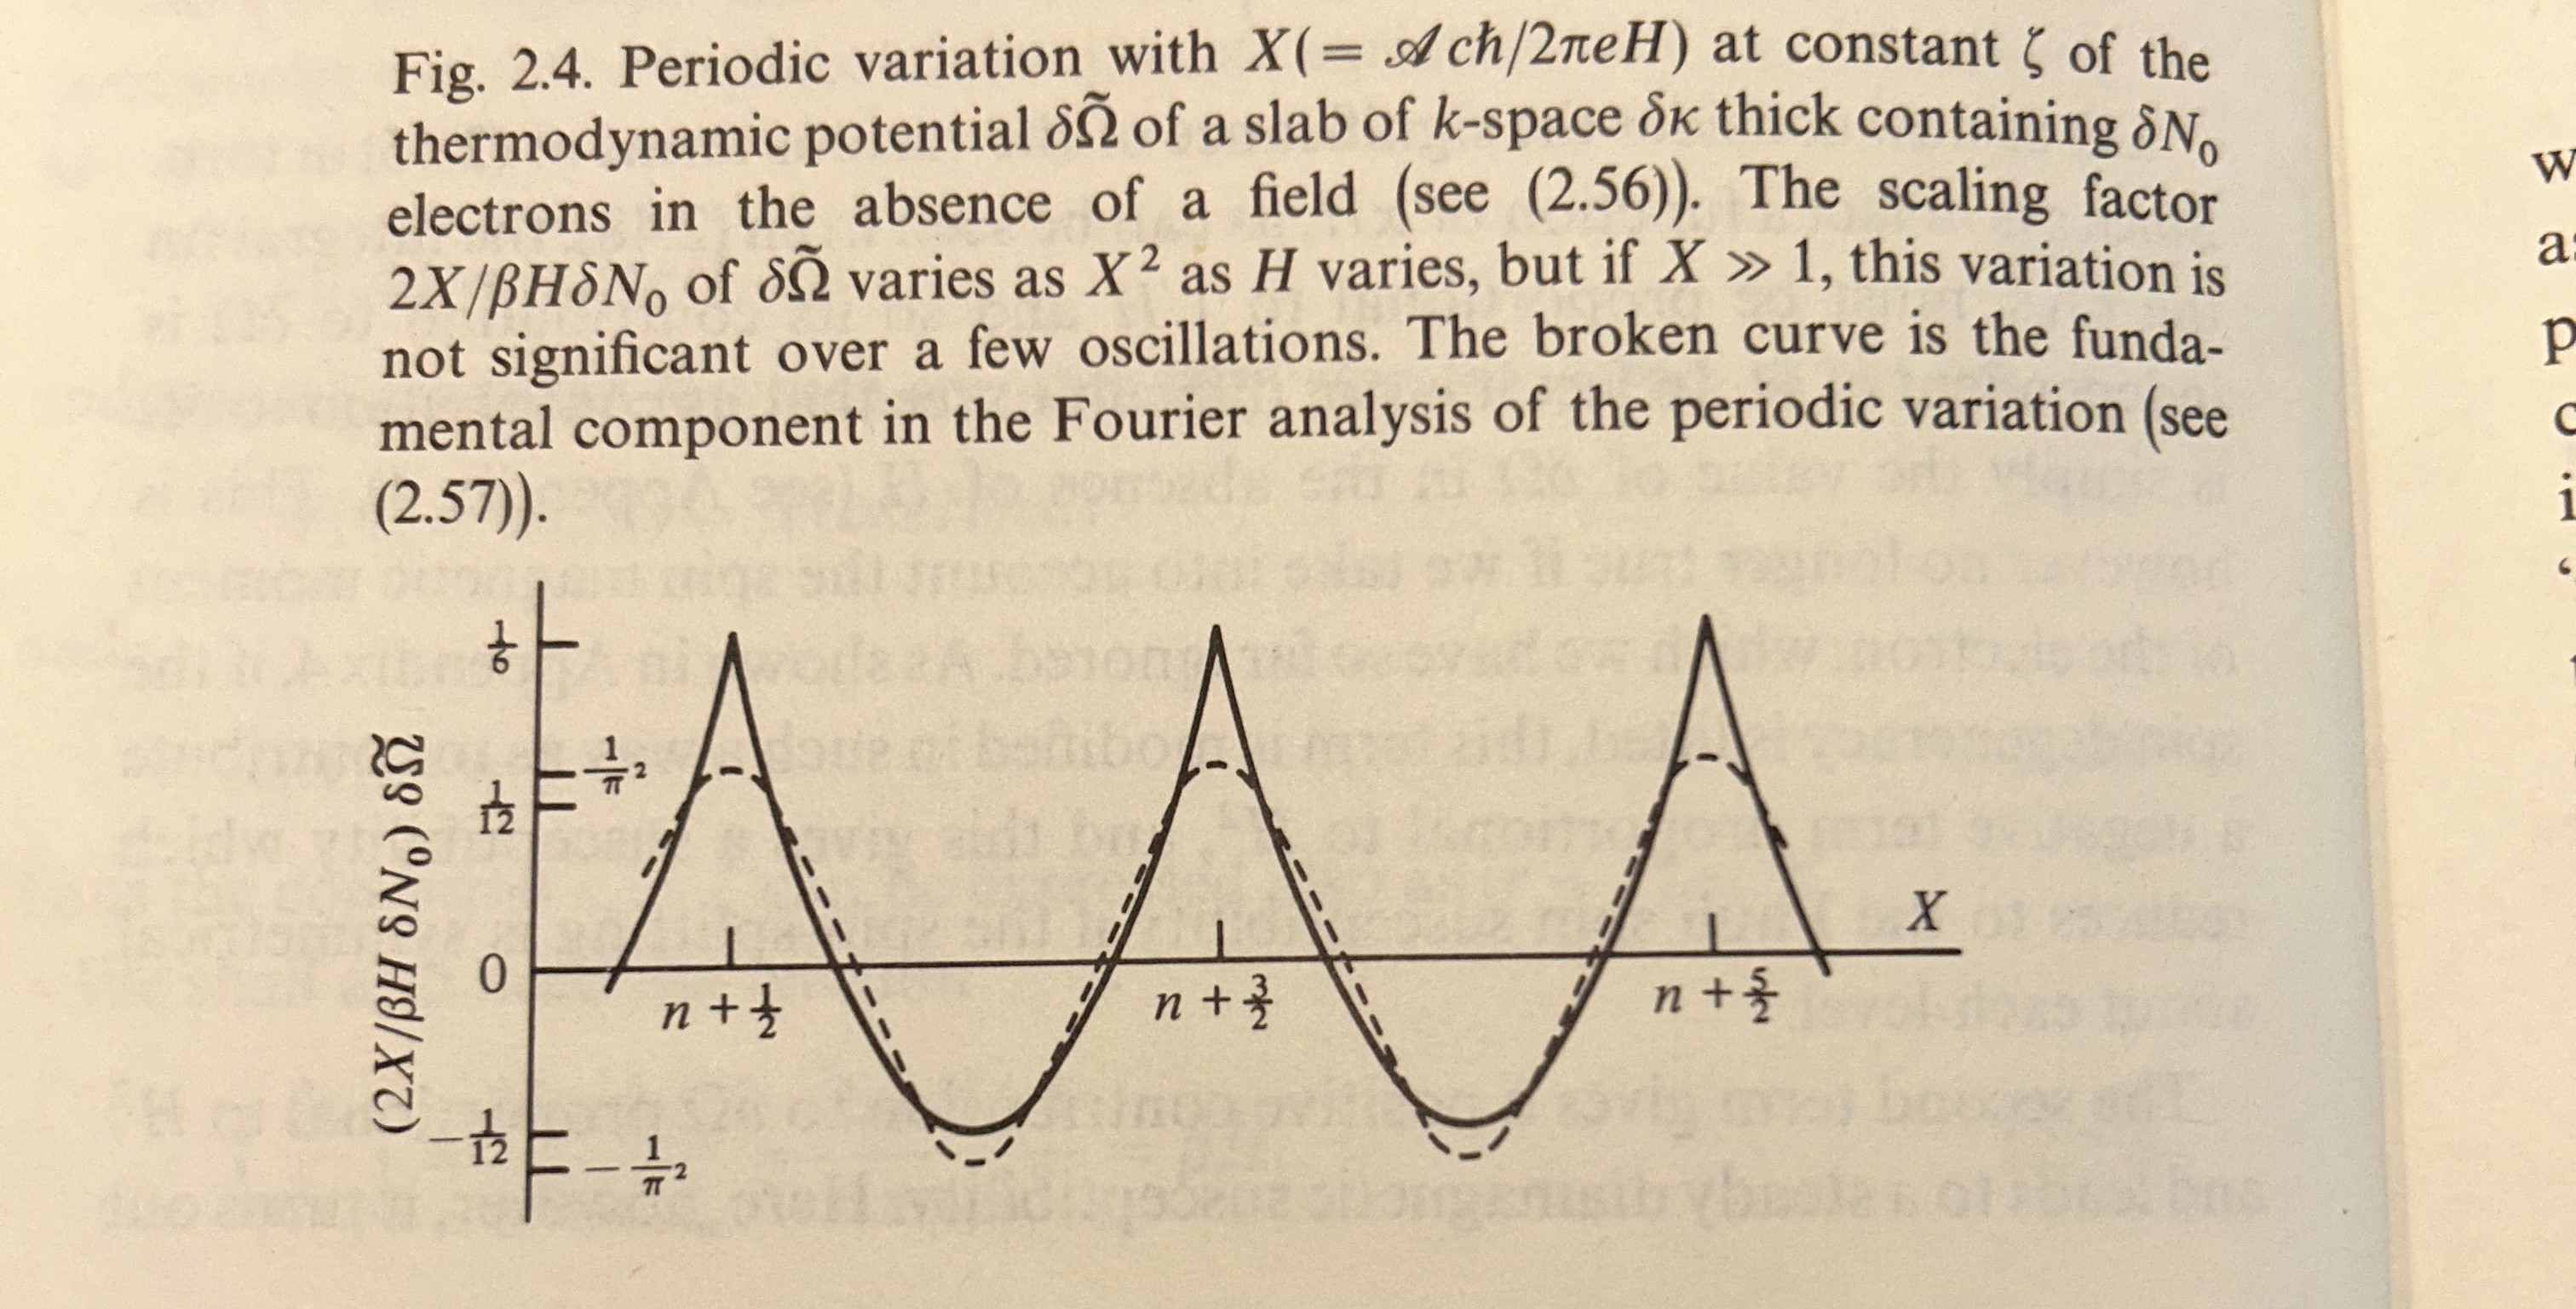
\includegraphics[width=0.75\textwidth]{figures/oscillations_free_energy.jpg}
\caption{Oscillations of our thermodynamic potential $\delta\Omega$ with $X$.  Taken from \textit{Magnetic Oscillations in Metals}.}
\label{fig:oscillations-energy}
\end{figure}

\subsection{Calculation of magnetisation}

Recall that the magnetic moment parallel to $H$, in our $T=0$ contribution, is given by
\begin{equation}
    \delta \tilde{M} = -\left( \frac{\partial(\delta\tilde{\Omega})}{\partial H} \right)_\zeta.
\end{equation}

We can also define our (two-dimensional) Fermi surface from Eqn. \ref{eqn:area-n}, 
\begin{equation}
    \mathcal{A} := A(X) = \frac{2\pi eH}{\hbar}X.
\end{equation}

So when we are taking our $\partial_H$ derivative, we will have
\begin{equation}
    X = \frac{\hbar\mathcal{A}}{2\pi e}\frac{1}{H} \implies \frac{\partial X}{\partial H} = -\frac{\hbar\mathcal{A}}{2\pi e} \frac{1}{H^2}
\end{equation}

we can safely ignore the $H^2$ term out front as it simply will yield a term proportional to $H \propto 1/X$ times our bracket terms in Eqn. \ref{eqn:potential-step}.  While it immediately seems that is not justified, since we have a term proportional to $X^2$ in square brackets, this is fine because the terms in square brackets are actually bounded!  The $N$ term constantly gets redefined as $X$ increases, meaning that the $1/X$ prefactor will kill that term for large enough $X$.  This is more easily seen through the Fourier series version, where we obtain a factor of $1/X$ times a sum over cosine terms.  So assuming our $H^2$ prefactor is constant, taking the (negative) derivative of our expressions lead to
\begin{equation}
    \boxed{ \delta \tilde{M} = \frac{\beta\mathcal{A}V\delta\kappa}{4\pi^3} \big[ X - (N+1) \big] = \beta \, \delta N_0\big[ X - (N+1) \big]}
\end{equation}

where $\delta N_0 := \mathcal{A}V\delta\kappa/4\pi^3$ is the number of particles in the two-dimensional slab for $H=0$ for any particular value of $\mathcal{A}$; however our particular value of $\mathcal{A}$ or $\zeta$ may actually change with $H$.  We can take this derivative for our Fourier series expression too, which yields
\begin{equation}
    \boxed{ \delta \tilde{M} = -\beta \delta N_0 \sum_{p=1}^\infty \frac{\sin\big[ 2\pi  p(X - 1/2) \big]}{\pi p} }
\end{equation}

While we have shown that our magnetization will oscillate, also shown pictorially in Fig. \ref{fig:oscillations-mag}, we have not show how it has anything to do with our Fermi surface area $\mathcal{A}_\text{FS}$ (which is the whole reason we are studying it).  Recall that $x = n + 1/2$ when taking our discretized Landau level energies; $X$ is defined as the $x$ for our fermi level.  Thus from Eqn. \ref{eqn:area-n}, we have the area of our FS 
\begin{equation}
    \mathcal{A}_\text{FS} = \frac{2\pi eH X}{\hbar} \implies X = \frac{\hbar \mathcal{A}_\text{FS}}{2\pi eH}.
\end{equation}

As our magnetization is oscillatory in $X$, it must be oscillatory in $\hbar\mathcal{A}_\text{FS}/2\pi eH$.  So looking at the oscillations of $\delta \tilde{M}$ as a function of $1/H$ can experimentally determine the area of our FS!

\begin{figure}[tb]
\centering
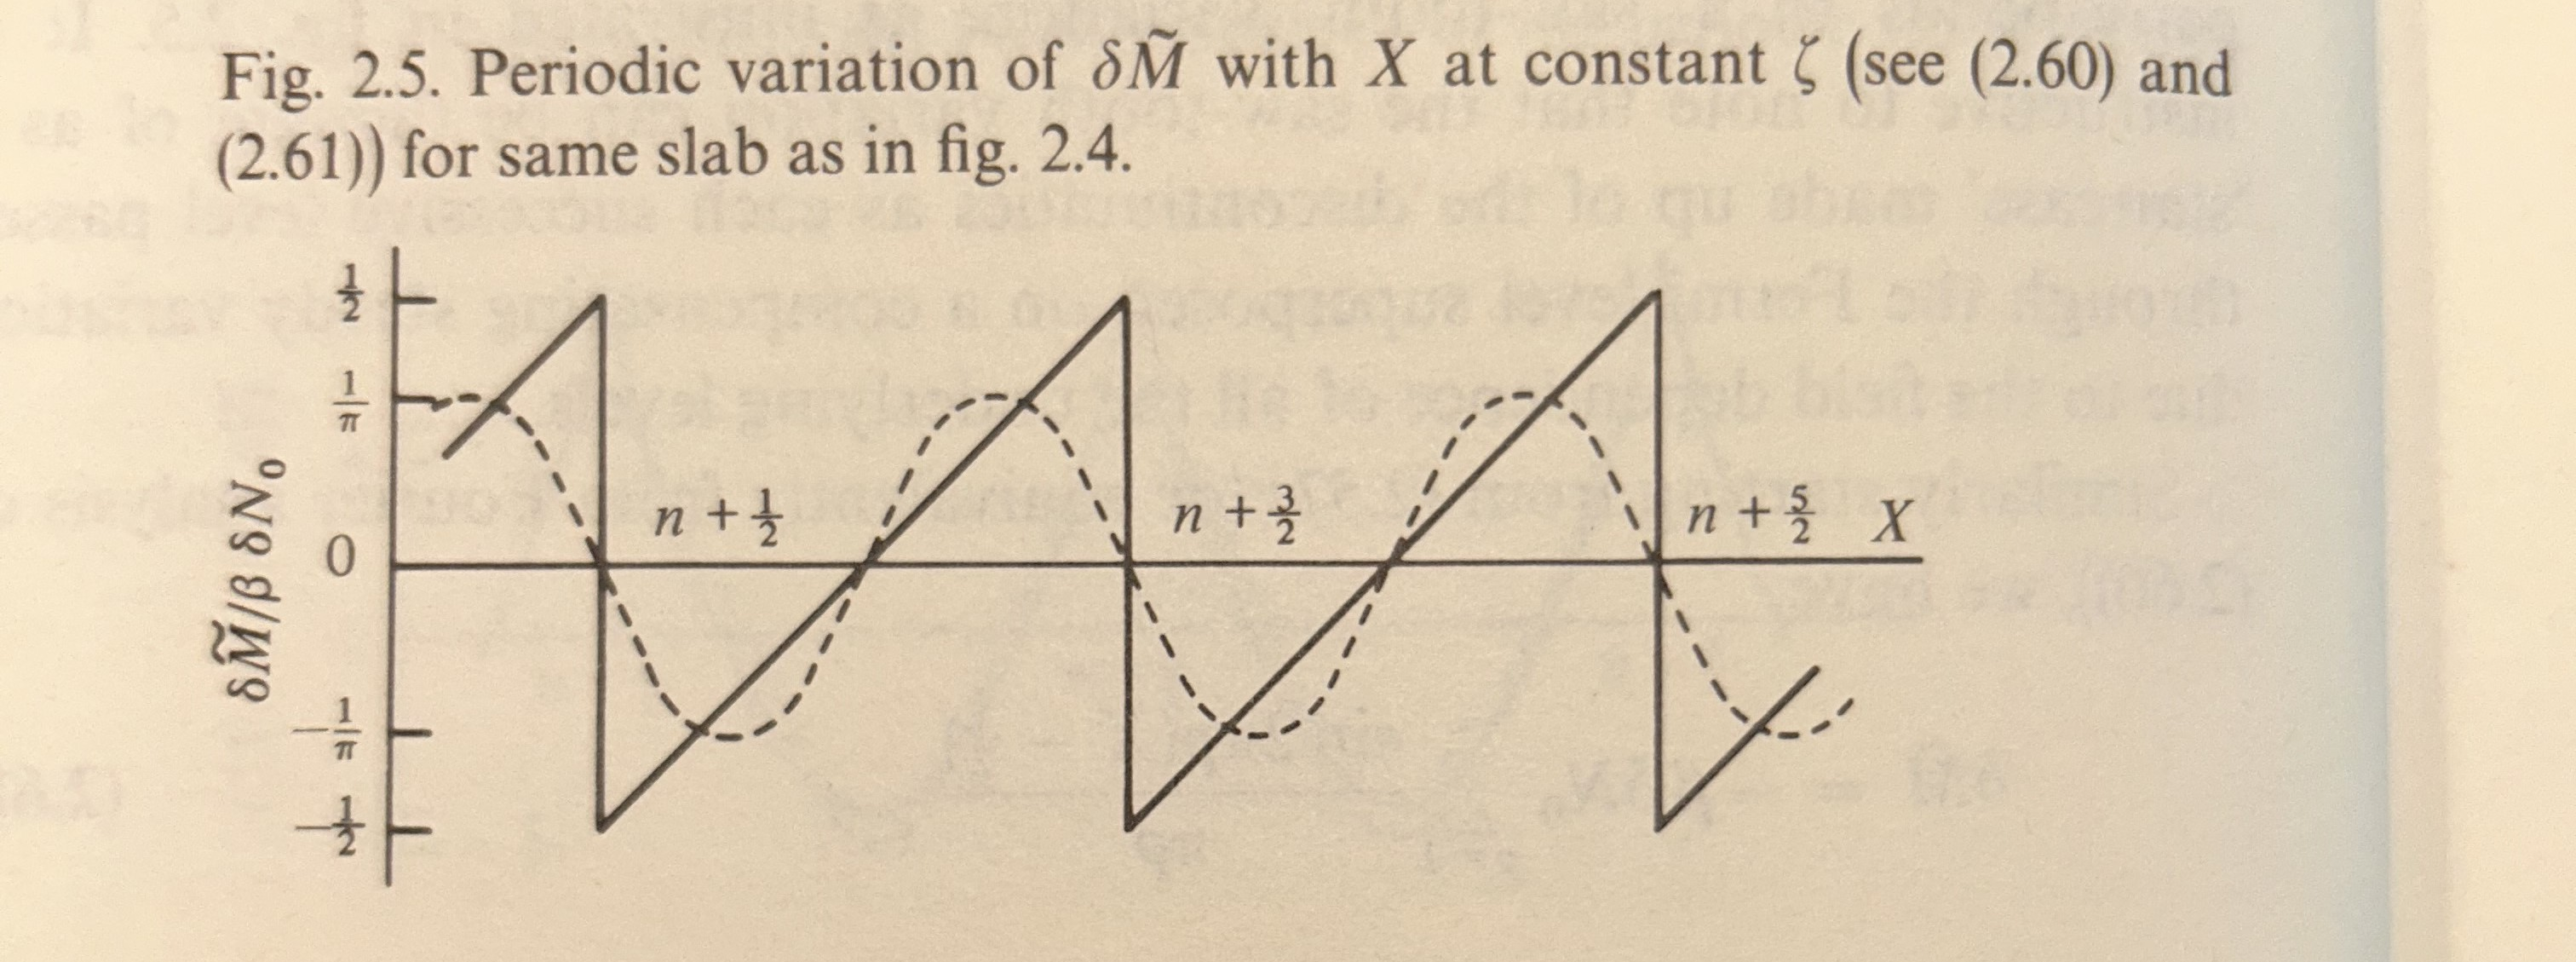
\includegraphics[width=0.75\textwidth]{figures/oscillations_magnetization.jpg}
\caption{Oscillations of our magnetization $\delta \tilde{M}$ with $X$.  Taken from \textit{Magnetic Oscillations in Metals}.}
\label{fig:oscillations-mag}
\end{figure}

\subsubsection*{What is the big picture?}
It is important to think now about where these oscillations actually come from.  Working backwards, all of our important terms here arise from our $\Delta$ dependent terms.  Since $\Delta := X - (N + 1/2)$, this physically represents the energy difference between the highest occupied Landau level and the actual fermi level.  Since that is constantly changing as our tubes cross our Fermi surface, that gives rise to oscillations in our magnetisation through the oscillations in our thermodynamic potential $\Omega$.  

\newpage
\section{Appendix: Group velocity of a given state}

\em I originally had this above, but these notes ended up being longer than expected.  Thus I am moving this to the end here for the sake of space. \em 
\par

We want to justify the use of $\mathbf{v} = \hbar^{-1}\partial_\mathbf{k}\epsilon_\mathbf{k}$ when looking at some electron in our metal.
\par

We will now prove (and then use) the Hellmann-Feynman theorem.  For some parameter $\lambda$, we will consider $H_\lambda |\psi_\lambda\rangle = E_\lambda |\psi_\lambda \rangle$.  Through the product rule, and assuming a normalized wavefunction, we can multiply by $\langle \psi_\lambda|$ and take the derivative with respect to $\lambda$.
\begin{align}
    \frac{dE_\lambda}{d\lambda} &= \frac{d}{d\lambda}\langle \psi_\lambda | H_\lambda | \psi_\lambda\rangle \\
    &= \left\langle \frac{d\psi_\lambda}{d\lambda} \bigg| H_\lambda \bigg| \psi_\lambda \right\rangle + \left\langle \psi_\lambda \bigg| \frac{dH_\lambda}{d\lambda} \bigg| \psi_\lambda \right\rangle + \left\langle \psi_\lambda \bigg| H_\lambda \bigg| \frac{d\psi_\lambda}{d\lambda} \right\rangle \\
    &= E_\lambda \left\langle \frac{d\psi_\lambda}{d\lambda} \bigg| \psi_\lambda \right\rangle + \left\langle \psi_\lambda \bigg| \frac{dH_\lambda}{d\lambda} \bigg| \psi_\lambda \right\rangle + E_\lambda \left\langle \psi_\lambda \bigg| \frac{d\psi_\lambda}{d\lambda} \right\rangle \\
    &= E_\lambda \frac{d}{d\lambda} \langle \psi_\lambda | \psi_\lambda \rangle + \left\langle \psi_\lambda \bigg| \frac{dH_\lambda}{d\lambda} \bigg| \psi_\lambda \right\rangle \\
    &= \left\langle \psi_\lambda \bigg| \frac{dH_\lambda}{d\lambda} \bigg| \psi_\lambda \right\rangle
\end{align}

as $\langle \psi_\lambda | \psi_\lambda \rangle=1$ is constant by construction.  Since we typically work in $\mathbf{k}$-space, we typically have $\lambda \mapsto \mathbf{k}$.  We then will use the $\mathbf{k}\cdot\mathbf{p}$ Hamiltonian ($H^{kp}$, which acts on the periodic part of a Bloch function $|u_{n\mathbf{k}}\rangle$)
\begin{equation}
    H^{kp} = \frac{(\hbar\mathbf{k} + \mathbf{p})^2}{2m} + V := H_0 + H_\mathbf{k}'.
\end{equation}

where
\begin{equation}
    H_0 = \frac{p^2}{2m} + V \quad \text{ and } \quad H_\mathbf{k}' = \frac{\hbar^2 k^2}{2m} + \frac{\hbar \mathbf{k}\cdot\mathbf{p}}{2m}.
\end{equation}

We typically split these terms up and use perturbation theory on $H_\mathbf{k}'$, however for our case of taking a derivative with respect to $\mathbf{k}$ we see
\begin{equation}
    \frac{dE_\mathbf{k}}{d\mathbf{k}} = \left\langle u_{n\mathbf{k}} \bigg| \frac{d H^{kp}}{d\mathbf{k}} \bigg| u_{n\mathbf{k}} \right\rangle = \left\langle u_{n\mathbf{k}} \bigg| \frac{d H_\mathbf{k}'}{d\mathbf{k}} \bigg| u_{n\mathbf{k}} \right\rangle = \left\langle u_{n\mathbf{k}} \bigg| \frac{\hbar^2 \mathbf{k}}{m} + \frac{\hbar\mathbf{p}}{m} \bigg| u_{n\mathbf{k}} \right\rangle.
\end{equation}

Then note how $[\partial_j,e^{-i\mathbf{k}\cdot\mathbf{r}}]f = (-ik_je^{i\mathbf{k}\cdot\mathbf{r}}f + e^{-i\mathbf{k}\cdot\mathbf{r}}\partial_j f) - e^{-i\mathbf{k}\cdot\mathbf{r}}\partial_j f = -ik_je^{-i\mathbf{k}\cdot\mathbf{r}}f$ with our test function $f$.  So $[\mathbf{p},e^{-i\mathbf{k}\cdot\mathbf{r}}] = (-i\hbar)(-i)\mathbf{k}e^{-i\mathbf{k}\cdot\mathbf{r}} = -\hbar\mathbf{k}e^{-i\mathbf{k}\cdot\mathbf{r}}$.  Since our full wavefunction is $|\psi_{n\mathbf{k}}\rangle = e^{i\mathbf{k}\cdot\mathbf{r}}|u_{n\mathbf{k}}\rangle$,
\begin{align}
    \frac{dE_\mathbf{k}}{d\mathbf{k}} &= \left\langle u_{n\mathbf{k}} \bigg| \left(\frac{\hbar^2 \mathbf{k}}{m} + \frac{\hbar\mathbf{p}}{m}\right) e^{-i\mathbf{k}\cdot\mathbf{r}}e^{i\mathbf{k}\cdot\mathbf{r}} \bigg| u_{n\mathbf{k}} \right\rangle \\
    &= \left\langle u_{n\mathbf{k}} \bigg|e^{-i\mathbf{k}\cdot\mathbf{r}} \left(\frac{\hbar^2 \mathbf{k}}{m} - \frac{\hbar^2 \mathbf{k}}{m} + \frac{\hbar\mathbf{p}}{m}\right) e^{i\mathbf{k}\cdot\mathbf{r}} \bigg| u_{n\mathbf{k}} \right\rangle \\
    &= \hbar\left\langle \psi_{n\mathbf{k}} \bigg| \frac{\mathbf{p}}{m} \bigg| \psi_{n\mathbf{k}} \right\rangle.
\end{align}

Since the expectation value on the RHS is our average (group) velocity for our electron, we have shown that $\mathbf{v} = \hbar^{-1}\partial_\mathbf{k}\epsilon_\mathbf{k}$.

\end{document}